\section{Approach}
\begin{figure*}[]
 \centering
  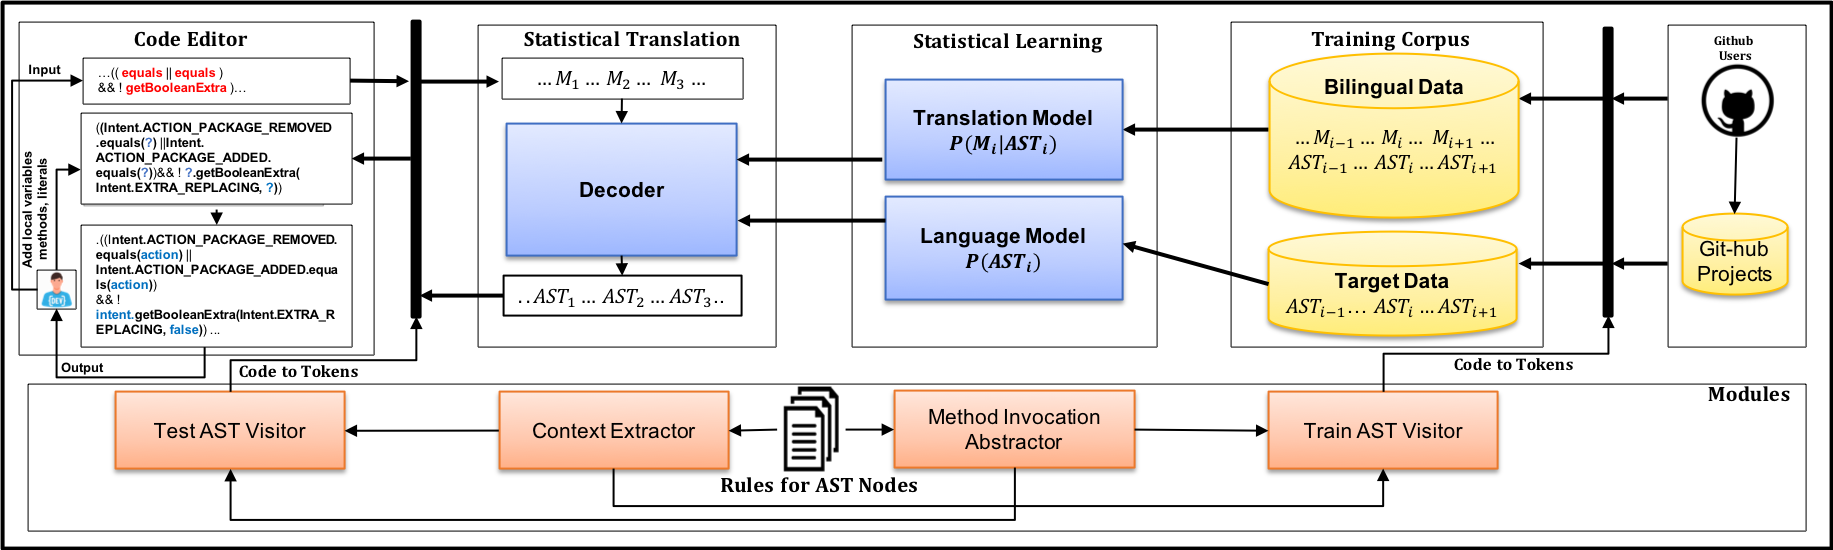
\includegraphics[width=\linewidth]{ApproachOverview.png}
  \caption{Overview Approach of InvocMap }
  \label{fig:ApproachOverview}
\end{figure*}
We summarize the engines inside InvocMap on Figure \ref{fig:ApproachOverview}. From developer view, InvocMap provides a plugin inside with Java code editor to allow (s)he to write a single or multiple method names inside the code environment. From this input, InvocMap translates each method names to respective ASTs. These ASTs reflect the complex structure of method invocations which might be inconvenient for developers to remember. They were abstracted at level 3 in our definition, means they only require developers to add local variables, local methods or literals to get the final code. We will discuss about MI at level 3 of abstraction in the next section. The ability of inferring ASTs for code completion relies on the Statistical Translation module. The training process is done by the Statistical Learning module. This module learns information from the data extracted from large scale Github code corpus  \cite{id:Github}. In general, our statistical approach takes advantages of the knowledge of implementing MIs of experience developers, representing it by a machine learning model to help non-experience developers in retrieving effective implementation of MIs. Both the source code at developers side and code corpus are analyzed to extract sequences of tokens by the Train AST Visitor and Test AST Visitor module we developed. Inside these visitors, we handle each AST Node types by function of modules Context Extractor and MI Abstractor, which we discuss in next sections.
\subsection{Levels of MI Abstraction in InvocMap}
In this section, we describe our theorems for method invocation abstraction.
\begin{definition}
Level 1 of abstraction of a method invocation is the information about method name of that method invocation.
\end{definition}
\begin{definition}
Level 2 of abstraction of a method invocation is the information about type (or signature) of that method invocation.
\end{definition}
\begin{definition}
Level 3 of abstraction of a method invocation is the Abstract Syntax Tree of that method invocation with abstracted place holder for local variables, local methods and literal.
\end{definition}
\begin{definition}
Level 4 of abstraction of a method invocation is the complete Abstract Syntax Tree of that method invocation.
\end{definition}
Along with 4 levels of abstraction in MI, we have the definition of local context provided for each MI. 
\begin{definition}
Local Context of a method invocation is the information about types of local entities and suggested terms. Local entities are local variables, local method invocations and literals inside the MI. The suggested terms are the words that appeared inside the MI.`
\end{definition}

An example of how we see 4 levels is shown in Figure \ref{fig:mapping_expression}. In this code snippet, we have level 1 as method name \texttt{println}. The level 2 of abstraction brings us information about type, which is \texttt{java.io.PrintStream.println}.The level 4 is the final source code which is compilable. The layer 3 is the AST that is having 2 places which are local entities are abstracted by their type information. In the implementation, we represent this AST in level 3 by 4 fields: the code with abstracted places for local entities, the list of types of required arguments to add, the list of imported APIs and the type of MI. These 4 fields will make an unique identification for the expression, which will serve as a representative token for the AST. Because of this, when developer receives an AST at level 3 of abstraction, (s)he will know what types of local variables (s)he can get to get the final code, along with the set of imported APIs. In our work, we focus on the inference from level 1 to level 3 by translation.
We will use information of local context to help developers who already remember what variables should run inside the MI and some words inside the MI to better retrieve the AST of implementation. In Figure \ref{fig:mapping_expression}, we see 2 local entities, including the string literal \texttt{"index"} and the integer variable \texttt{i}. The suggested terms can be \texttt{"System"} and \texttt{"+"} sign. 



\subsection{Levels of Abstraction in Other AST Nodes}
In the context of this work, we call other AST Nodes as all kinds of AST except the MI that are defined in \cite{id:ASTDocumentation}.
\begin{definition}
Level 1 of abstraction of other AST Nodes is the information about the Partial Qualified Name (PQN) of type of those nodes.
\end{definition}
\begin{definition}
Level 2 of abstraction of other AST Nodes is the information about Fully Qualified Name (FQN) of type of those nodes.
\end{definition}
According to definition in \cite{8453132}, an example is the API \texttt{java.io.File}. In this API, we have \texttt{File} as PQN while we have \texttt{java.io.File} as FQN.

\subsubsection{Source and Target Tokens for Other AST Nodes}
We extract information about other AST Nodes to provide useful context for MIs prediction. In the source language, we extract all tokens of level 1 of abstraction for each AST Node, and extract all tokens in level 2 of that AST Node to put into target language. The implementation of the extraction is the Context Extractor module, which is called inside Train AST Visitor and Test AST Visitor. 

\subsubsection{Source and Target Tokens for Method Invocations}
 There are two types of information we want to embed for MI: the mapping between method name and the AST and the information relate to local context. For the first type of information, the source language will store information about token as level 1 of abstraction of MI, while the target language stores information about level 3 of abstraction of MI. Besides, information about local context will be stored by level 1 of abstraction in the source and level 2 of abstraction in the target language. A sequence of tokens for MI in Figure \ref{fig:mapping_expression} is shown in Figure \ref{fig:method_desc_example}.
 \noindent
\begin{figure}
    \centering
      \begin{subfigure}{0.23\textwidth}
        \center{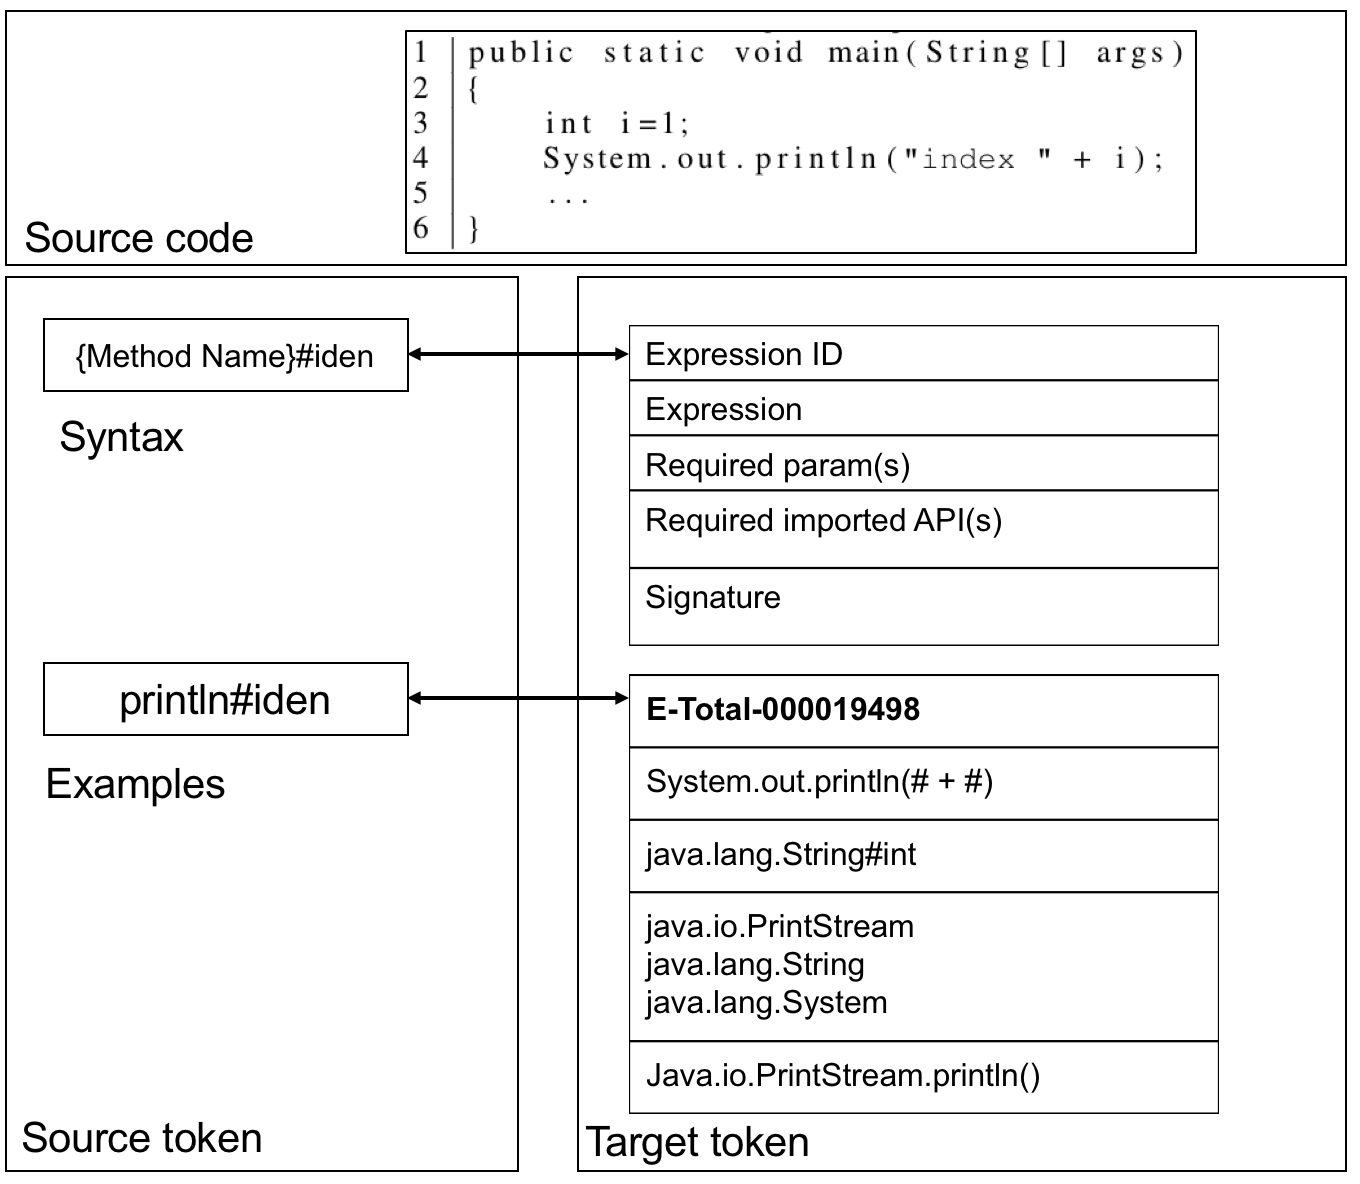
\includegraphics[width=\linewidth]
        {images/example_source_target.png}}
        \caption{Example of AST\_Level3 instance}
        \label{fig:mapping_expression} 
      \end{subfigure}
      \hfill
      \begin{subfigure}[t]{0.23\textwidth}
        \center{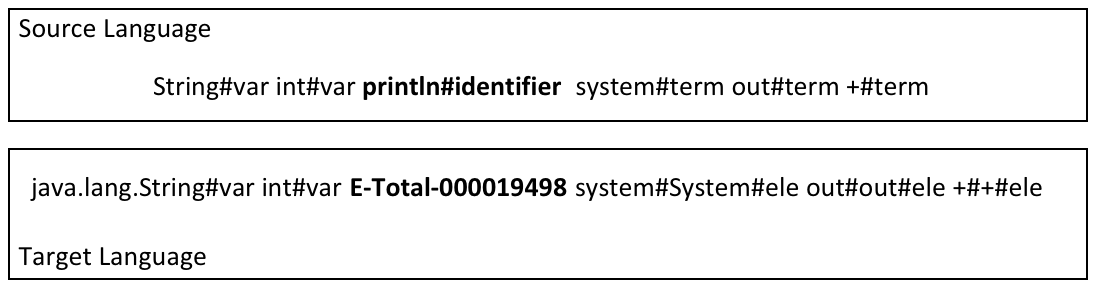
\includegraphics[width=\linewidth]
        {images/methodDescription_example.png}}
        \caption{Example of method name tokens in source and MI object tokens at level 3 in target language}
        \label{fig:method_desc_example}
      \end{subfigure}
      \hfill
      \begin{subfigure}{0.5\textwidth}
        \center{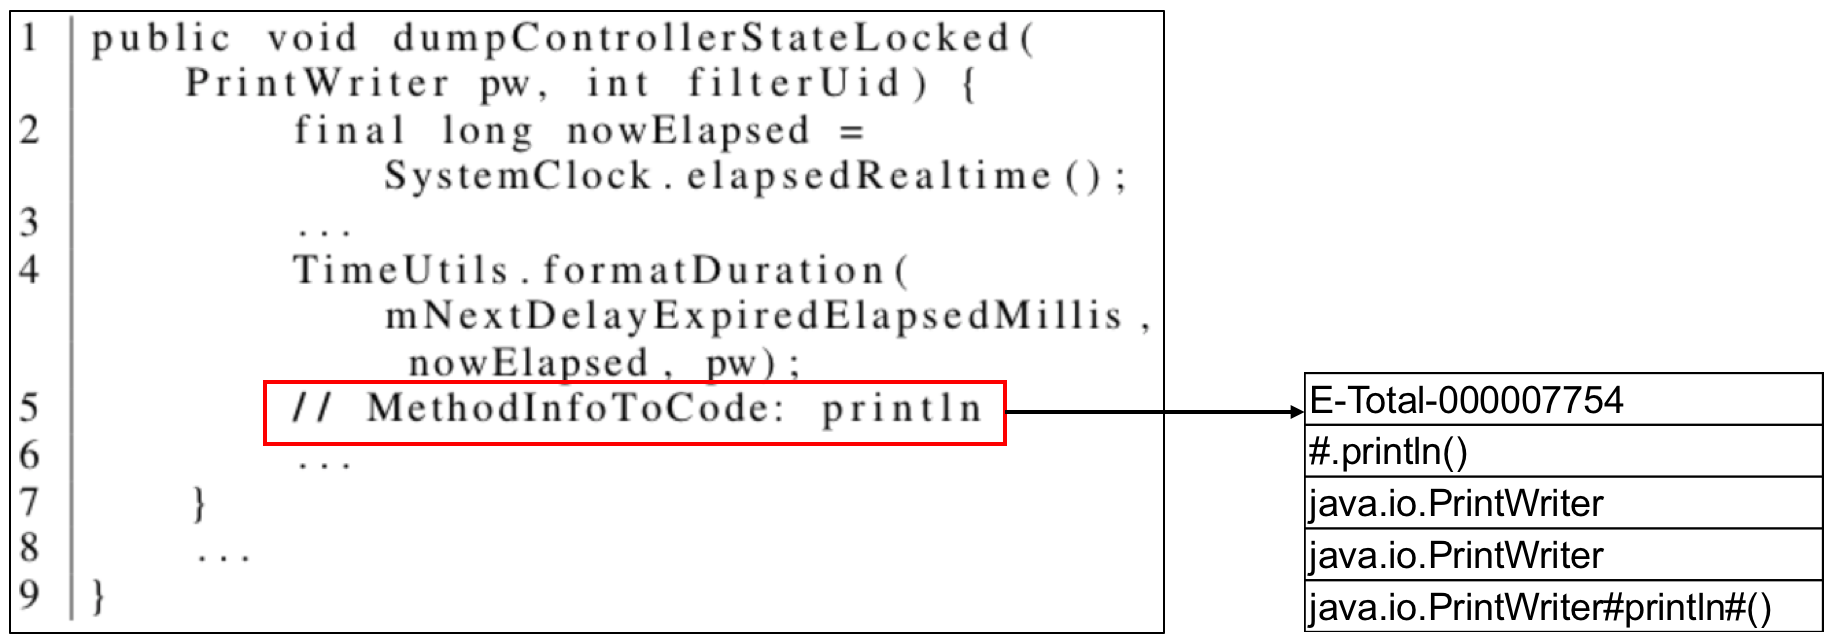
\includegraphics[width=\linewidth]
        {images/example_in.png}}
        \caption{\label{fig:example_in} Example of inference from method name to MI at level 3 for code snippet in \cite{id:IntrinsicAndroidExample}}
      \end{subfigure}
\caption{
\label{fig:CombineImageOfASTLevel3}%
Representations of AST\_Level3}
\end{figure}

\subsubsection{Method Invocation Abstraction}
\begin{lstlisting}[basicstyle=\tiny,caption={Algorithm for Method Invocation Abstraction},label={lt:AlgorithmMethodAbstractor}]
AST_Level3 abstractMethodInvocation(
		mi : MethodInvocation ,
		dictionaryAST : Set<AST_Level3>,
		visitor : MICVisitor) {
	AST_Level3 result=new AST_Level3(mi);		
	visitor.result=result;
	
	//visit receiver if exist
	Expression receiverExpr=getReceiver(mi);		
	if(receiverExpr not null)
		visitor.visit(receiverExpr);
	
	// add method name and open parenthesis
	result.strCode.append(getMethodName(mi)+"(");
	
	// visit content of arguments
	Expression[] listArguments=getParams(mi);		
	for each Expression argExpr in listArguments:
		visitor.visit(argExpr);
	
	// add close parenthesis
	result.strCode.append(")");

	// set uniqueId
	setUniqueId(result,dictionaryAST);
	
	return result;		
}
...
class AST_Level3 {
	// field to store AST in level 3
	strCode : String;

	// Other informations need to 
	//	add to get final code
	listArguments : List<Type>;
	setImportedAPIs : Set<Type>;	
	strSignature : Type;

	// id is created by the uniqueness of 4 other fields 
	uniqueId : String;
	
}
...
class MICVisitor extends ASTVisitor{
	result : AST_level3;
	...		
	void visit(ASTNode node) {
		/*
		 * If visit local entity,
		 * mark as a place holder
		 * in the AST structure
		 */
		if(isLocalEntity(node)) {
			result.strCode.append("#");
			result.listArguments.append(getType(node));				
		} 
		else  {	
			// visit structure and update result
			// can be recursive if node have children nodes
			visitStructure(node);
		} 			
		// In every cases, add type of node to set of imported APIs
		result.setImportedAPIs.add(getType(node));		
	}	
}
\end{lstlisting}
We get information about level 3 of abstraction in MI by proposing an algorithm in Listings \ref{lt:AlgorithmMethodAbstractor} and \ref{lt:AlgorithmMethodAbstractorPartB}. The \texttt{abstractMethodInvocation()} function is invoked when the Train AST Visitor or Test AST Visitor visit a MI and return the abstraction in level 3 by an instance of AST\_Level3 class. This function will use the child class of ASTVisitor called InvocAbstractVisitor defined in Listing \ref{lt:AlgorithmMethodAbstractor} (Line \#45). This visitor will visit each element inside the MI, check and abstract if the element is a local entity. This visitor also stores other information about the code of AST, the list of required types for each local entities and the set of imported APIs. The handling strategy for each types of AST Node inside the MI is implemented in the \texttt{visitStructure()} function in  Listing \ref{lt:AlgorithmMethodAbstractorPartB}(\#32). After visiting and abstracting of MI to an \texttt{AST\_Level3}, this object is checked by the first four fields defined in Listing \ref{lt:AlgorithmMethodAbstractorPartB}(\#1-\#10)  to see if its exist in the dictionary or not. If yes, it will have the id of the existing object in the dictionary. Otherwise, it will generate a new unique id and will be added to the dictionary. The dictionary stores information about abstraction at layer 3 of MIs in the training step. An example of  \texttt{AST\_Level3} object is shown in Figure \ref{fig:mapping_expression}.


\subsection{SMT}
To learn the mapping between source and target language, we apply the PBMT \cite{Green2014}. This approach works based on the ability to learn from two models: the language model and the translation model.
\subsubsection{Language Model}
Language Model (LM) plays an important role in a PBMT system. LM is used to predict the next token given a sequence of previous tokens \cite{Koehn:2003:SPT:1073445.1073462}. The more comprehensive corpus of target language do we have, the LM model quality for prediction is higher. LM had been used widely in Software Engineering (SE) researches \cite{Hindle:2012:NS:2337223.2337322,Hel:7180076,Liu:7883371} with potential results. The most basic LM in NLP is uni-gram LM, which calculates the probability of each word based on the number of the appearance of that word in the corpus. This LM provides drawbacks that it doesn't take into account the history of how a word was used in a sequence from previous words. However, if we calculate the probability of a word from all previous words in a sequence of translation, the cost for doing such evaluation is expensive (\cite{Jurafsky:2009:SLP:1214993}). 
\\
Here we use the n-gram language model, which proposed in \cite{Jurafsky:2009:SLP:1214993}. The n-gram LM is used to measure the probability of implementation of MI given a list of previous implementations. The n-gram LM overcome the cost of measuring history for each word by considering and approximate the history for the last n-words that appeared before the current word. Assume that we have m tokens in the target language \({AST_{1},...,AST_{m}}\), the probability provided by LM is:

\begin{equation} 
\tiny
\label{eq:EQ_Probability}
 P[AST_{1}, ...,AST_{m}]=\prod_{i=1}^{m}P[AST_{i} | AST_{i-n},...,AST_{i-1}]
\end{equation}

In equation \ref{eq:EQ_Probability}, the probability for each element of the production on the right side is estimated by the co-occurrence of the current word given the list of the previous words in the target corpus (\cite{Jurafsky:2009:SLP:1214993}). In our model, we use 4-gram LM as the default configuration of LM in NLP.

\subsubsection{Translation Model}
The translation model calculates the probability of a phrase from source language that can be translated to a phrase in a target language. In our problem, if we have a sentence   \({D}\) as the translated result of sentence \({S}\) as tokens in the source language, the selection of \({D}\) as the best candidate is calculated as follows:

\begin{equation} 
\tiny
\label{eq:EQ_Argmax}
 D_{best}=argmax_{D}(p(S|D)*P_{LM}(D)))
\end{equation}

In equation \ref{eq:EQ_Argmax}, \({p(S|D)}\) is the probability of translation model to get the best accuracy calculated by the work of \ref{eq:EQ_ProbTransModel}. In this formula, \(I\) is the number of phrase appeared in sentence \({D}\), while \(\theta ({s_{i}}|{d_{i}})\) is the probability functions between phrase calculated by \cite{Green2014}. Compare to the original translation between natural languages, the translation model in NL has an another type of distribution called reordering distribution. Since our corpus has consistent length between source and target, we don't apply this distribution to equation \ref{eq:EQ_ProbTransModel}.
\begin{equation} 
\tiny
\label{eq:EQ_ProbTransModel}
{p(S|D)=\prod_{i=1}^{I} \theta ({s_{i}}|{d_{i}}) }
\end{equation}


